\documentclass{article}
\usepackage[utf8]{inputenc}
\usepackage{graphicx}

\title{test}
\author{Lauren Corlies}
\date{February 2019}

\begin{document}

\maketitle

\section{Introduction}
Here's some words

\section{Adding Some Stuff}
Hooray for words!

\subsection{Make sure this works!}
Why would you do this to me Mac?! Why?!

\subsection{A new section}
to test a push to git!

\subsection{Now I'm editing directly on my computer!}
I've added some more words!

\section{Trying the rich test option}
\subsection{there are keywords for section and subsection}
\begin{enumerate}
\item Adding in a list
\item is SO 
\item MUCH
\item EASIER
\end{enumerate}

WOOOOO!

\begin{figure}
    \centering
    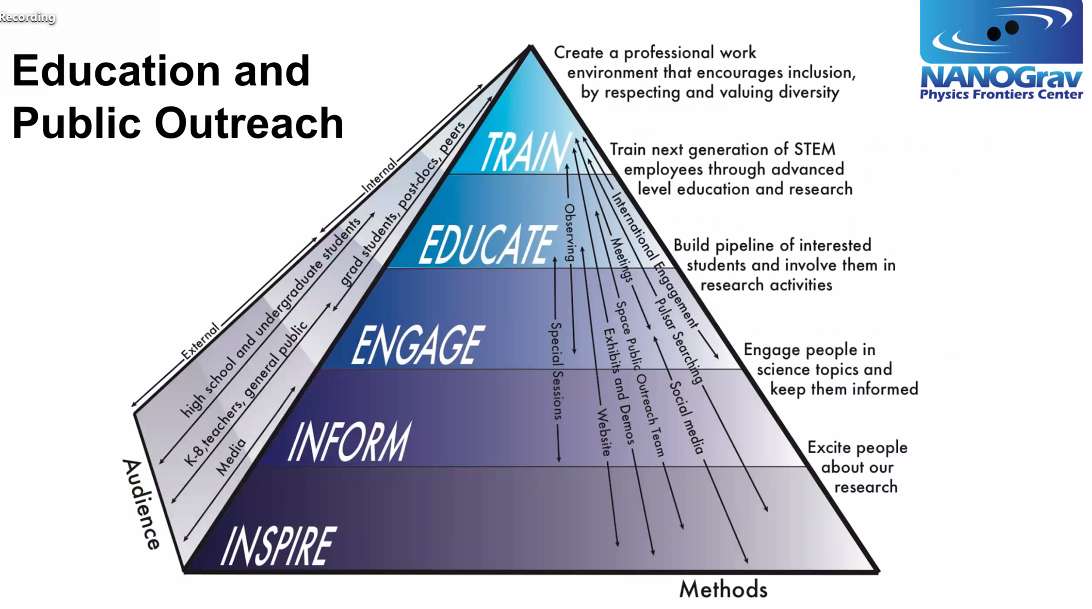
\includegraphics[width=1.0\textwidth]{first_figure.png}
    \caption{Testing out to see what happens with the git sync}
    \label{fig:first}
\end{figure}

\section{Branch Push take 2!}
TRYING to push to the new-branch again. Let's see if it works

\end{document}
